%------------------------------------------------------------------------------
% Sam Nazari
% Spring 2016: Manuscript for journal submission
%------------------------------------------------------------------------------
%
% AMS-LaTeX version 2 sample file for journals, based on amsart.cls.
%
\documentclass{amsart}
%     If your article includes graphics, uncomment this command.
\usepackage[]{graphicx}
\usepackage[text={7in,10in},centering]{geometry}
\usepackage{color}
\usepackage{amsmath}
\usepackage{amssymb}
\usepackage[linesnumbered,ruled]{algorithm2e}
\usepackage{amsfonts}
\usepackage{graphicx}
\usepackage{hyperref}
\usepackage{float}
\usepackage{caption}
\usepackage{tikz}
\usepackage{setspace} % Double spaceing
\doublespacing
\usepackage{subcaption}
\hypersetup{
    bookmarks=true,         % show bookmarks bar?
    unicode=false,          % non-Latin characters in Acrobat’s bookmarks
    pdftoolbar=true,        % show Acrobat’s toolbar?
    pdfmenubar=true,        % show Acrobat’s menu?
    pdffitwindow=false,     % window fit to page when opened
    pdfstartview={FitH},    % fits the width of the page to the window
    pdftitle={Unknown Input Observer Examples},    % title
    pdfauthor={Sam Nazari},     % author
    pdfsubject={UIO},   % subject of the document
    pdfcreator={Sam Nazari},   % creator of the document
    pdfproducer={Sam Nazari}, % producer of the document
    pdfkeywords={keyword1} {key2} {key3}, % list of keywords
    pdfnewwindow=true,      % links in new PDF window
    colorlinks=false,       % false: boxed links; true: colored links
    linkcolor=red,          % color of internal links (change box color with linkbordercolor)
    citecolor=green,        % color of links to bibliography
    filecolor=magenta,      % color of file links
    urlcolor=cyan           % color of external links
}

\newtheorem{theorem}{Theorem}
\newtheorem{lemma}{Lemma}
\newtheorem{prop}{Proposition}
\theoremstyle{definition}
\newtheorem{definition}{Definition}
\newtheorem{example}[theorem]{Example}
\newtheorem{xca}[theorem]{Exercise}
\newtheorem{app}{Application}
\newtheorem{ass}{Assumption}
\newtheorem{cond}{Condition}
\newtheorem{problem}{Problem}

\theoremstyle{remark}
\newtheorem{remark}{Remark}

\numberwithin{equation}{section}

%    Absolute value notation
\newcommand{\abs}[1]{\lvert#1\rvert}

%    Circled numbers
\newcommand*\circled[1]{\tikz[baseline=(char.base)]{
            \node[shape=circle,draw,inner sep=2pt] (char) {#1};}}
            
%    Blank box placeholder for figures (to avoid requiring any
%    particular graphics capabilities for printing this document).
\newcommand{\blankbox}[2]{%
  \parbox{\columnwidth}{\centering
%    Set fboxsep to 0 so that the actual size of the box will match the
%    given measurements more closely.
    \setlength{\fboxsep}{0pt}%
    \fbox{\raisebox{0pt}[#2]{\hspace{#1}}}%
  }%
}

\sloppy
\definecolor{lightgray}{gray}{0.5}
\setlength{\parindent}{0pt}

\def\X{b}
\def\tX{\tilde{b}}
\def\mX{B}
\def\tmX{\tilde{B}}
\def\bone{{\bf 1}}
\def\bzero{{\bf 0}}
\def\bx{{\bf x}}
\def\by{{\bf y}}
\def\bz{{\bf z}}
\def\bof{{\bf f}}
\def\N{\mathbb{N}}
\def\Z{\mathbb{Z}}
\def\Q{\mathbb{Q}}
\def\R{\mathbb{R}}
\def\C{\mathbb{C}}
\def\mP{\mathbb{P}}
\def\mE{\mathbb{E}}
\def\mI{\mathbb{I}}
\def\cN{\mathcal{N}}
\def\cV{\mathcal{V}}
\def\cE{\mathcal{E}}
\def\cC{\mathcal{C}}
\def\cT{{\cal T}}
\def\cB{{\cal B}}
\def\eps{\epsilon}
\def\reff{\textup{Reff}}
\def\deg{\textup{deg}}

\begin{document}

\title{Maximum Attack Tolerance by Optimal Spectral Expansion}
% \title{Maximum Attack Tolerance by Spectral Expansion Optimization}

%    Information for first author
\author{Sam Nazari}
%    Address of record for the research reported here
\address{Northeastern University}
%    Current address
%\curraddr{Department of Mathematics and Statistics,
%Case Western Reserve University, Cleveland, Ohio 43403}
\email{nazari@ece.neu.edu}
%    \thanks will become a 1st page footnote.
%\thanks{The first author was supported in part by NSF Grant \#000000.}

%    Information for second author
%\author{Author Two}
%\address{Mathematical Research Section, School of Mathematical Sciences,
%Australian National University, Canberra ACT 2601, Australia}
%\email{two@maths.univ.edu.au}
%\thanks{Support information for the second author.}

%    General info
%\subjclass[2000]{Primary 54C40, 14E20; Secondary 46E25, 20C20}

\date{07-February-2016}

%\dedicatory{This paper is dedicated to our advisors.}

\keywords{Spectral Expansion, Expanders, Intruder Detection, Robust Graph Topologies.}

\begin{abstract}
Let $G=(\cV,\cE_G)$ be a network consisting of $n$ agents such that $k < n$ of the agents are malicious intruders and let $H=(\cV,\cE_H)$ be a subgraph embedded in $G$ consisting of agents equipped with detection filters to identify intrusions by malicious agents. Assume that $G$ is also under attack from an external adversary whose goal is to disconnect the largest set of vertices in $G$ from $H$ by sabotaging $\epsilon$ fraction of its edge set, leaving the detection filters unable to sense intrusions from malicious agents. 

% The aim of the adversary is to cut $G$ so that the monitoring agents spanned by $H$ are unable to detect intrusions by malicious agents in the rest of $G$. 

% Let $G=(V,E_G)$ be the topology of a network consisting of $n$ agents under attack from external adversaries and let $H=(V,E_H)$ be a subgraph embedded in $G$ consisting of agents equipped with detection filters to identify network intrusions by malicious agents. The goal of the adversaries is to disconnect the largest set of the vertices from the network by sabotaging $\epsilon$ fraction of its edge set so that the malicious agents can disrupt network operations in an undetected manner while the agents endowed with detection filters aim to monitor $G$ for such activities from malicious agents. 

This paper establishes the algebraic and combinatorial conditions for which $H$ is maximally robust to attacks from external adversaries.  
% %The problem considered in this paper is that of identifying the structure of $H$ such that it is maximally robust to attacks from adversaries. 
% %This paper establishes algebraic and combinatorial conditions for which $H$ is maximally robust to attacks from adversaries. 
It is shown that the algebraic conditions are a relaxation of the corresponding combinatorial conditions, and that extracting a robust topology for $H$ can be formulated as an optimization problem involving the Laplacian spectrum of $G$. A spectral algorithm is provided to recover the desired topology and two design procedures are given for $H$ with the property that after an $\epsilon$ fraction of the edges are adversarially removed, the network still maintains a connected component that spans at least $(1-\frac{\epsilon}{2h})$ fraction of the vertices, with $h$ denoting the edge expansion of $G$. For the class of similar graphs that are isospectral, we relate the algebraic connectivity to the third moment of the adjacency matrix of $G$, providing an alternative means for obtaining $H$ instead of through spectral means. 

% We aim to recover the largest hidden expander, $H$, in $G$ (by spectral methods?).

% It is also shown that the problem of assessing the reliability of the monitoring network is related to the number of triangles incident on the vertices of the graph spanned by the monitoring agents.   

     
% We consider the topology of distributed agents tasked with detecting and identifying simultaneous attacks from intelligent adversaries. The adversaries can disrupt the network, $G=(V,E_G)$, by sabotaging $\epsilon |E_G|$ fraction of the links, rendering a subset $S \subseteq V$ of the network nodes isolated. 
% Under this setting, a graph invariant, $h(G)$, is defined that naturally relates the network connectivity and diameter to the graph spectrum. An SDP is formulated to recover the induced subgraph, $H(V,E_H)$ that is maximally robust to attacks from malicious agents. Two design procedures are provided for choosing the edge set of $H$ with the property that after an $\epsilon |E_G|$ fraction of the edges are adversarially removed, the network still maintains a connected component that spans at least $(1-\frac{\epsilon}{2h}) |V|$ fraction of the vertices.
% We consider the problem of designing the topology of a network with distributed agents tasked with detecting and identifying simultaneous attacks from intelligent adversaries. The adversaries can disrupt the network, $G=(V,E_G)$, by sabotaging $\epsilon |E_G|$ fraction of the links, rendering a subset $S \subseteq V$ of the network nodes isolated. 

% Under this setting, a graph invariant, $h(G)$, is defined that naturally relates the network connectivity and diameter to the graph spectrum. An SDP is formulated to recover the induced subgraph, $H(V,E_H)$ that is maximally robust to attacks from malicious agents. Two design procedures are provided for choosing the edge set of $H$ with the property that after an $\epsilon |E_G|$ fraction of the edges are adversarially removed, the network still maintains a connected component that spans at least $(1-\frac{\epsilon}{2h}) |V|$ fraction of the vertices.
% We consider the problem of designing the topology of a network with distributed agents tasked to detect and identify simultaneous attacks from intelligent adversaries.  It is assumed that the adversaries can disrupt network communications by sabotaging links and that they can attack the nodes in an unrestricted fashion. 

% Under this setting, we define a graph invariant that is a measure of the network resiliency and we relate this quantity to the Laplacian spectrum of the network. Furthermore, an SDP is provided so that for any given topology, $G=(V,E_G)$, an induced subgraph, $H=(V,E_H)$, is obtained which is maximally robust to attacks from malicious agents. Additionally, two explicit constructions of $H=(V,E_H)$ are provided with the property that after an $\epsilon$ fraction of the edges are adversarially removed, the network still maintains a connected component that spans at least $(1-\frac{\epsilon}{2h})$ fraction of the vertices. 
% We consider the problem of designing a network of distributed agents to detect and identify simultaneous attacks from malicious agents. It is shown that the problem of choosing the network topology that is maximally robust to attacks from malicious agents is related to the spectrum of a specially constructed monitoring graph. Two constructions are provided with the property that after an $\epsilon$ fraction of the edges are adversarially removed, the network still maintains a connected component that spans at least $(1-\frac{\epsilon}{2h})$ fraction of the vertices. It is also shown that the problem of assessing the reliability of the monitoring network is related to the number of triangles incident on the vertices of the graph spanned by the monitoring agents. 
\end{abstract}

\maketitle

% %-----------Introduction--------------
\section{Introduction}
Modern society has grown dependent on critical infrastructure systems that are fundamentally networked. These distributed systems are interconnected due to the existence of local information pathways between parties. Today, the design and operation of such complex networked systems involves multidisciplinary teams and a major consideration is the evaluation of vulnerabilities that can lead to unexpected service disruptions in critical infrastructures. Commonly cited examples of critical infrastructure systems include data, transportation, financial, social, sensor and water distribution networks, not to mention power grids and biological systems. Indeed, the prevalence of distributed, interconnected systems in critical infrastructure has been a major area of research and development for the past decade.    

\medskip

A notable consideration in designing such systems is that of the network \textit{resilience}\cite{Akoglu2015,Dinh2015,Grubesic2008,Murray2008,Banerjee2009,Banerjee2011,Pinar2010,Albert2004,Basar2012,Dinh2012,Agarwal2013,Dinh2010,Thai2015,Shen2012,Rieg2009,Bai2012,Rieg2012,Basar2011,Kis2013,Dong2014,Basar2012,Basar2013,Geh2013,Dong2013,Lamport1982,Meng2014,Garcia2014,Cheng2015,Pas2015,Pas2013,Pas2012,PasPhd2012,Pas2010,Pas2007,Kha2014,Gupta2010,Fawzi2014,Wente2014,Sund2013,Teix2014}

Roughly speaking, A resilient system is one that maintains an accepted level of operational normalcy in response to disturbances, including threats of an unexpected and malicious nature \cite{Rieg2009}. 

a resilient system is any system with the property that after undergoing an unexpected disturbance (or attack), an acceptable level of normal operation can maintained (or recovered) without major system structural reconfiguration.  

Roughly,a graph is considered robust, if it is capable of retaining its structural and connectivity properties after the loss of an $\epsilon$ portion of its edge set.  Although key vertices are routinely attacked by malicious agents, local failures  do not always  lead  to  the  loss  of  overall information transmission in the network. 

\medskip

Evaluating network vulnerabilities is an important consideration for designers because unmitigated risks to the system can lead to service disruptions in critical infrastructure. 

background, motivation and literature review.
The problem of finding cuts with small spectral expansion is an open problem in theoretical computer science. The small-set expansion conjecture 

\medskip

In \cite{Akoglu2015}, the authors consider the problem of extracting the most robust local subgraph. 

\medskip

In \cite{Van2013}, the authors consider the problem of finding the critical region of a planar graph whose removal would lead to the highest network disruption. They show that only a polynomially bounded number of regions need to be evaluated to ascertain the critical region. The authors also use percolation theory to quantitatively characterize an attack on the critical region.   
\medskip
The main contributions of this paper are as follows. We introduce a spectral framework for network resiliency analysis that quantifies attacks from malicious agents both within the network and from external adversaries. We show that the combinatorial problem of finding the network topology that is maximally resilient to external attacks is equivalent to an unconstrained optimization problem involving the spectral expansion of a subgraph within the network. With respect to this formulation, we give an algorithm that recovers the subgraph of interest within a polynomial time factor of the number of vertices in the original network. Our framework assumes knowledge of the network spectral expansion a priori, an assumption that is not always met in real world applications. When this assumption is not met, we provide an alternative characterization of the subgraph $H$ that is maximally robust to attacks and is computable in linear time \cite{Sesh2015,Sesh2012,Tsour2011,Tsour2009}. In particular, a key relation between the spectral expansion of a network and the third moment of its adjacency matrix is derived. Finally, we provide algebraic approaches to constructing the subgraph of monitoring agents with guaranteed lower bounds on the spectral expansion to directly address the problem of designing the subgraph of maximal resiliency. 

% %-----------Background--------------
\section{Background}
\subsection{Graph Theory}
Graph theory has proven to be useful in a variety of diverse applications. Recently, graph theory has been used to model the interconnected nature of many networked control systems, multi-agent systems and cyber-physical systems. In this section, we provide a rudimentary background to graph theory. The interested reader is referred to \cite{Dies} for an elaborate treatment.

\medskip

We denote a graph by $G = (\mathcal{V},\mathcal{E})$, where $\mathcal{V} = \{1,\ldots, n\} \in \mathbb{N}$ is the \textit{vertex set} and $\mathcal{E} \subseteq \mathcal{V} \times \mathcal{V}$ is the \textit{edge set}. We assume all graphs are simple, finite, and undirected.  We denote by $xy \in \mathcal{E}(G)$ the edge $xy$ that is in the edge set of the graph $G$. In this case, $x$ and $y$ are considered to be \textit{adjacent or neighboring} vertices.  If all the vertices of $G$ are pairwise adjacent, then $G$ is complete.  A complete graph on $n$ vertices is denoted by $K_n$.  If $G$ is an undirected graph and a subset of the vertices, $S \subset \cV$, forms a complete graph, the then subgraph induced by $S$ is known as a \textit{clique}. The number of vertices in a graph is the \textit{order}, usually denoted by $|G|=n$. A vertex, $a$, is \textit{incident} with an edge, $e=(c,a)$, if $a \in e$.  Then we say that $e$ \textit{joins} $c$ and $a$, the \textit{endvertices}.

\medskip

The set of \textit{neighbors} of the vertex $v \in \mathcal{V}(G)$ is denoted by $\mathcal{N}_v$. The notation $|\mathcal{N}_v|=m$ denotes the cardinality of the set of neighbors of $v$, in this case $m$. The \textit{degree} of a vertex $v$ is the number of edges that the vertex $v$ participates in $d_v := |\{w: (vw) \in \mathcal{E}(G)\}|$. If every vertex has the same degree,$d$, then we say $G$ is a $d$-regular graph and denote this by $G_d$. 

\medskip

Consider $G = (\mathcal{V},\mathcal{E})$. Define $x$ as a mapping from the vertex space of $G$ to the reals, $x: \mathcal{V}(G) \rightarrow \mathbb{R}$. Similarly, define $y$ as a mapping from the edge space of $G$ to the reals, $y: \mathcal{E}(G) \rightarrow \mathbb{R}$. The mappings $x$ and $y$, associate with each vertex (or edge) a scalar numeric value from the reals. 

\medskip

Consider the linear operator $A:\mathbb{R}^n \rightarrow \mathbb{R}^n$. When we apply $A$ to $x$, the resulting value at a vertex $a$ is the sum of the values of the function $x$ over all the neighbors, $b$, of $a$.  Hence the action of the operator $A_G$ on $x$ at $a$ can be captured as $(A x)(a) = \sum_{b:(ab) \in \mathcal{E}} x(b)$. We refer to $A_G$ as the \textit{adjacency matrix} of $G$. It is usually defined: 
\begin{align*}
 A_{ij}= 
\begin{cases}
    1,              & \text{if } ij\in \mathcal{E}\\
    0,              & \text{otherwise}
\end{cases}
\end{align*}
If $G_d$ is a $d$-regular graph, then it is slightly more convenient to work with its normalized adjacency matrix:
\begin{align*}
M = \frac{1}{d}A.
\end{align*}
We have the following relation between the combinatorial properties of $G_d$ and the eigenvalues of $M$:
\begin{lemma} \label{lem:eigA}
Let $G_d$ be a $d$-regular, undirected graph and let $M \in \R^{n \times n}$ be its normalized adjacency matrix. Let 
\begin{align*}
\mu_1 \geq \mu_2 \geq \ldots \geq \mu_n
\end{align*}
be the real eigenvalues of $M \in \R^{n \times n}$ with multiplicities. Then, 
\begin{enumerate}
\item $\mu_1 = 1$ and $\mu_n \geq -1$.
\item $\mu_2 = 1$ if and only if $G_d$ is disconnected.
\item $\mu_n = -1$ if and only if at least one of the connected components of $G_d$ is bipartite.
\end{enumerate}
\end{lemma}
\begin{proof}
The reader is referred to \cite{Dies} for the proof.
\end{proof}

If $G_d$ is a $d$-regular graph, then it is slightly more convenient to work with its normalized Laplacian matrix:
\begin{align*}
L = I-\frac{1}{d}A.
\end{align*}
The Laplacian of $G_d$ has many notable properties.  Here, we only note that $L$ is a symmetric, positive semidefinite, diagonally dominant, M-matrix. We have the following relation between the combinatorial properties of $G_d$ and the eigenvalues of $L$:
\begin{lemma} \label{lem:eigL}
Let $G_d$ be a $d$-regular, undirected graph and let $L \in \R^{n \times n}$ be its normalized Laplacian matrix. Let 
\begin{align*}
\lambda_1 \leq \lambda_2 \leq \ldots \leq \lambda_n
\end{align*}
be the real eigenvalues of $L \in \R^{n \times n}$ with multiplicities. Then, 
\begin{enumerate}
\item $\lambda_1 = 0$ and $\lambda_n \leq 2$.
\item $\lambda_k = 0$ if and only if $G_d$ has $k$ connected components.
\item $\lambda_n = 2$ if and only if at least one of the connected components of $G_d$ is bipartite.
\end{enumerate}
\end{lemma}
\begin{proof}
The reader is referred to \cite{Dies} for the proof.
\end{proof}
Finally, we state the variational characterization of the eigenvalues of a real symmetric matrix. 
\begin{lemma}[Variational Characterization of Eigenvalues] \label{lem:variational}
Let $L \in \R^{n \times n}$ be a real symmetric matrix and let 
\begin{align*}
\lambda_1 \leq \lambda_2 \leq \ldots \leq \lambda_n
\end{align*}
be its real eigenvalues, counted with multiplicities and sorted in increasing order. Let $\bof_1 \ldots \bof_k, k\leq n$ be orthonormal vectors such that $L\bof_i = \lambda_i \bof_i$ for $i = 1\ldots k$. Then,
\begin{align}
\lambda_{k+1} =\min_{\bof \in \R^{n} - \{0\}: \bof \bot \bof_1, \ldots, \bof \perp \bof_k} \quad \frac{\bof^T L \bof}{\bof^T \bof},
\end{align}
and any minimizer is an eigenvector of $\lambda_{k+1}$.
\end{lemma}
\begin{proof}
The reader is referred to \cite{Hor99} for the proof.
\end{proof}
\subsection{Edge Expansion, Cheegers Inequality \& Edge Density}
\begin{figure}
    \centering
    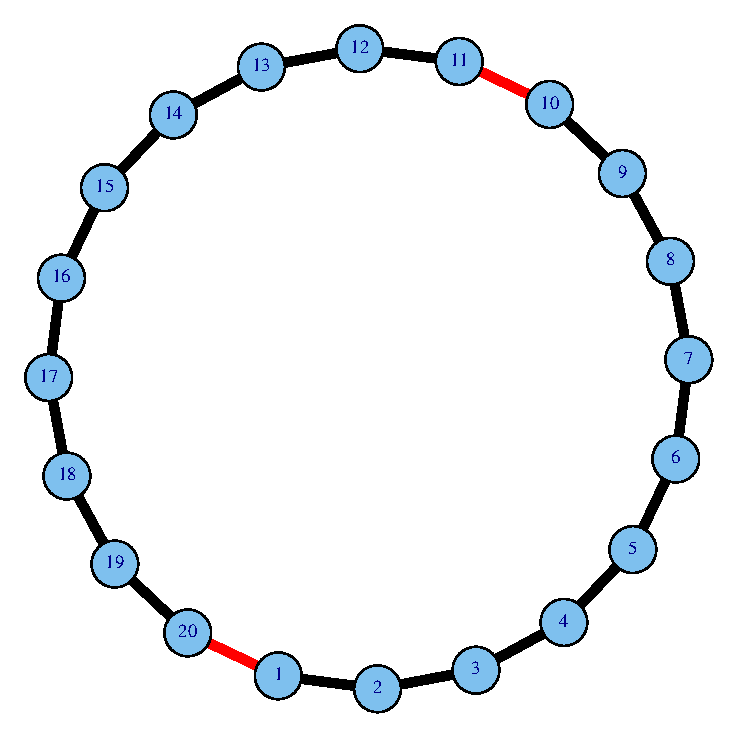
\includegraphics[scale=0.35]{ringGraph.eps}
    \caption{A ring graph with $n=20$. If this graph is cut at the edges that are colored red, then $n/2$ vertices of the graph will be disconnected. Since a large fraction of graph can be separated with only two cuts, we say that this graph does not have ``good expansion''.}
    \label{fig:ringGraph}
\end{figure}
In this section, we establish three results that relate the combinatorial invariants of $G$ to its spectral decomposition. We motivate the development of the results by considering the most reliable of all network topologies, the clique. In a clique, an adversary must remove a large fraction of the edges in order to disconnect a majority of the vertices from the graph. The clique is the gold standard of reliability in graphs, but unfortunately, it is also the least cost efficient approach because the number of edges in a clique over $n$ vertices is $\frac{n(n-1)}{2}$. The \textit{edge} and \textit{spectral expansions} are graph invariants that measure how much worse a graph is compared to a clique. 
\begin{definition}[Spectral Expansion] \label{def:specexp}
The \textit{spectral expansion} of a simple undirected graph $G$ is defined as the second smallest eigenvalue of $L$. 
\end{definition}
To define the \textit{edge expansion} of $G$ choose a subset of the vertices, $S$, and define the cut $\partial(S)=\{uv: u\in S, v \not\in S\}$ to be the set of edges that have one endpoint in $S$ and one endpoint not in $S$. Then the \textit{edge expansion} of the set $S$ can be defined as the ratio of the number of edges that leave $S$ to the number of vertices in $S$ normalized by $d$, i.e.:
\begin{definition}[Edge Expansion]\label{def:edgeexp}
The \textit{edge expansion} of the set $S$, for the cut $\partial (S)$, is defined as
\begin{align}\label{eq:expS} 
h(S) = \frac{\mid \partial(S)\mid}{d\cdot max\{\mid S \mid,\mid \bar{S}\mid\}}.
\end{align}
\end{definition}
On average, (\ref{eq:expS}) is the fraction of neighbors outside of the set $S$ for a randomly chosen element in the set $S$. It compares the actual number of edges that cross $\partial (S)$ to the maximum upper bound $d \mid S \mid$. Based on definition \ref{def:edgeexp}, the combinatorial expansion of $G$ is defined by the following optimization problem:
\begin{definition}[Combinatorial Expansion of $G_d$] \label{def:combexp} The \textit{combinatorial expansion} of a simple undirected graph $G$ is defined by: 
\begin{align} \label{eq:expG}
h(G) := \min_{\emptyset \subseteq \mid S \mid  \subseteq \frac{n}{2}} h(S).
\end{align}
\end{definition}
The combinatorial expansion, $h(G)$, is used in many applications that involve graph partitioning. Popular examples are clustering in data analysis and community detection in social networks. Computing the cut that minimizes $h(G)$, i.e. the optimal cut, is an NP-hard problem \cite{Garey1990}. Fortunately, it is possible to address the problem through spectral theory instead. In order to do this, however, there must be a relation between the spectral characterization of a graph and its combinatorial expansion. We now state the celebrated Cheeger inequality which precisely establishes this relation.
% Intuitively, the concept of edge expansion can be thought of in the following way. Consider a ring graph shown in Figure \ref{fig:ringGraph}. Deleting just two edges from the edge set of a ring graph leads to a disconnected graph. In particular, if the graph is cut at the right edges, then it is possible to disconnect $n/2$ vertices from the graph. Since cutting a small number of edges leads to a large number of vertices being disconnected in the graph, we say that the ring graph does not have ``good edge expansion''. Edge expansion is a combinatorial property of graphs that has been used to gauge graph connectivity and diameter (speed). 
\begin{theorem}[Cheeger's inequality] \label{thrm:cheeger}
For any graph $G$, we have
\begin{align}\label{eq:cheeger} 
\frac{\lambda_2(G)}{2} \leq h(G) \leq \sqrt{2 \lambda_2(G)}.	
\end{align}
\end{theorem}
\begin{proof}
The proof can be found in \cite{Chung97}
\end{proof}
The Cheeger inequality establishes a relationship between the spectral expansion of any graph, $\lambda_2 (G)$, and its combinatorial expansion, $h(G)$. If the graph spectrum is known, then it is easy to check whether or not the graph admits a sparse cut. Recall that Lemma \ref{lem:eigL} roughly states that the number of times that zero appears in the spectrum of $L_G$ is precisely the number of connected components of $G$. Therefore, $\lambda_2 (G) \approx 0$ implies $h(G) \approx 0$ and it can be concluded that the second smallest eigenvalue $\lambda_2 (G)$ and the expansion of a graph $h(G)$ are approximations of one another. 
In order to prove that a graph possess desirable expansion properties, one must show that the combinatorial expansion of the graph is bounded below by a constant. By the Cheeger inequality, then, it is enough to prove that the second smallest eigenvalue $\lambda_2$ for the family of graphs is bounded from below instead. Usually it is easier to reason about the eigenvalues of a graph than about its combinatorial expansion. Based on this reasoning, we define the notion of an expander graph next:
\begin{definition}[$\epsilon$-expander Graph]\label{def:expander}
We say $G_d$ is an $\epsilon$-\emph{expander} if $\lambda_2\geq \epsilon$.
\end{definition}
By analyzing the spectral properties of expander graphs it can be shown that they are essentially sparse graphs with the connectivity properties of complete graphs. \textcolor{red}{Can more be said here?} Given a cut $\partial (S)$, we may define another quantity that represents the density of edges between the set $S$ and its complement, $S^c = V-S$. This is known as the cut edge density: 
\begin{definition}[Edge Density of a cut].\label{def:edgedensity} The \textit{edge density} of a cut $\partial (S)$ is defined to be
\begin{align}\label{eq:edgedensity}
\rho (S) = \frac{\mid \partial(S) \mid}{\mid S \mid \mid S^c \mid}n.
\end{align}
\end{definition}
\begin{lemma}[Fallat Inequality]\label{lem:minedgedenalgconnect}
Let $G = (\cV,\cE)$ be a simple undirected graph. The edge density 
\begin{align*}
\rho (S) = \frac{\mid \partial(S) \mid}{\mid S \mid \mid S^c \mid}n
\end{align*}
of any subset of the vertex set, $S \subset V$, satisfies
\begin{align} \label{eq:edgDenIn}
\lambda_2 \leq \rho(S).
\end{align}
Furthermore, (\ref{eq:edgDenIn}) holds with equality for some cut $\partial (S)$ if the following conditions are satisfied: 
\begin{enumerate}
\item[i)] Each vertex $s \in S$ is adjacent to $d_1$ vertices in $S^c$ and each vertex $t \notin S$ is adjacent to $d_2$ vertices in $S$.
\item[ii)] $\displaystyle \frac{d_1}{d_2} = \frac{\mid S^c \mid}{\mid S \mid}$, 
\end{enumerate}
and the algebraic connectivity is then $\lambda_2 = \rho(S) = d_1+d_2$.
\end{lemma}
\begin{proof}
The reader is encouraged to consult \cite{Fallat2003} for the proof.
\end{proof}
\begin{figure}
    \centering
    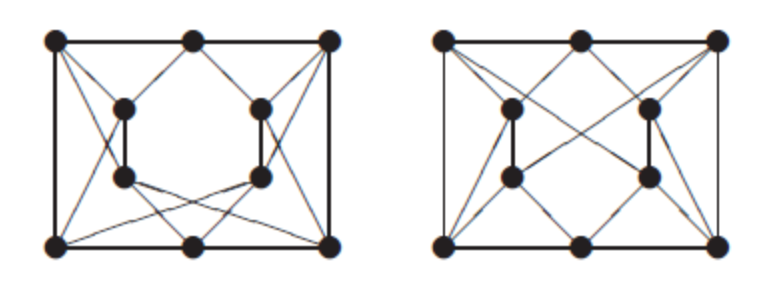
\includegraphics{cospectral.png}
    \caption{Two isospectral regular graphs with the same Laplacian and adjacency spectrum.}
    \label{fig:cospectral}
\end{figure}
It has been shown that matrix spectra do not uniquely determine graphs. For example, the two graphs in Figure \ref{fig:cospectral} are both 4-regular and share the same Laplacian and adjacency spectrum. However, they are not isomorphic graphs since the one on the right has more triangles than the one on the left. This line of reasoning leads us to relate graph invariants such as the number of triangles to the graph spectrum. 
\begin{theorem}[Algebraic Connectivity and Clustering Coefficient]\label{thrm:algTriangle}
Let $G = (\cV, \cE)$ be a simple undirected connected graph with $n$ vertices and $m$ edges. Then, 
\begin{align} \label{eq:nazInequality}
\frac{2m - R}{n-1} \leq \lambda_2 \leq \frac{n \displaystyle\sum_{i \in \cV}d_i^2 - 6n\triangle}{2mn - \displaystyle\sum_{i \in \cV} d_i^2}.
\end{align}
where $\triangle$ is the number of triangles in $G$ and
\begin{align*}
R = \sqrt[]{(n-2)\left ((n-1)\displaystyle\sum_{i \in \cV}d_i^2 + 2m(n-2m-1)\right)}.
\end{align*}
\end{theorem}
\begin{proof}
First we show $\displaystyle\frac{2m - R}{n-1} \leq \lambda_2$. The diagonal elements of $L$ and $L^2$ are $d_i$ and $d_i^2+d_i$ respectively. The latter is due to the fact that the sum of the rows of $L$ must equal $0$ and that the diagonal entries of $L^2$ are of the form $d_i^2 + \sum_{j\neq i}L_{ij}^2$. But the Laplacian matrix is defined over a binary field (0,1), therefore the summation term is the sum of $0$'s or $1$'s, so $\sum_{j\neq i}L_{ij}^2 = d_i$. Now, $\displaystyle\sum_{i \in \cV} d_i = 2m$ and $\displaystyle \sum_{i \in \cV}(d_i^2 + d_i) = \sum_{i \in \cV} d_i^2 + 2m$. Using the Cauchy-Schwarz inequality, one can show that $\displaystyle\sum_{i \in \cV} (d_i^2 + 2m) - \lambda_2^2 \geq \displaystyle\frac{(2m-\lambda_2)^2}{n-2}$. Carefully rearranging the terms will produce
\begin{align*}
\displaystyle\frac{2m - R}{n-1} \leq \lambda_2
\end{align*}
as desired. Next we show that $\lambda_2 \leq \frac{n \displaystyle\sum_{i \in \cV}d_i^2 - 6n\triangle}{2mn - \displaystyle\sum_{i \in \cV} d_i^2}$. Note that, by Lemma \ref{lem:minedgedenalgconnect}, $\displaystyle\lambda_2 \leq \rho(S)$. Let $S = \cN_i$. Observe that $\mid \partial (\cN_i) \mid = \displaystyle\sum_{j \in \cN_i} d_j - 2\triangle_i$, where $\triangle_i$ denotes the number of triangles that vertex $i$ participates in. The trick to realizing this is that $\cN_i$ is defined such that vertex $i$ is not included in the set. The set $\cN_i$ contains all the immediate neighbors of $i$ but not $i$ itself. Now, Lemma \ref{lem:minedgedenalgconnect} can be stated as
\begin{align*}
\lambda_2 \mid \cN_i \mid \mid V - \cN_i \mid \leq n \mid \partial(\cN_i) \mid.
\end{align*}
But the quantity $\mid \cN_i \mid \mid V - \cN_i \mid$ can be written as $d_i (n-d_i)$. Therefore, we have
\begin{align*}
\lambda_2 d_i (n-d_i) \leq n\displaystyle\sum_{j \in \cN_i} d_j - 2\triangle_i.
\end{align*}
Hence, by summing over all the vertices in the graph, one obtains:
\begin{align*}
\lambda_2 \leq \frac{n \displaystyle\sum_{i \in \cV}d_i^2 - 6n\triangle}{2mn - \displaystyle\sum_{i \in \cV} d_i^2}
\end{align*}
as desired. 
% Then $\displaystyle \lambda_2 \leq \displaystyle\frac{\mid \partial (\cN_i)\mid }{\mid \cN_i \mid \mid V - \cN_i \mid}n = \displaystyle\frac{\mid \partial (\cN_i)\mid }{d_i (n-d_i)}n$.
\end{proof}
\subsection{Distributed System Model}
\subsubsection{Nominal System Behavior} Consider a group of $n$ agents with single integrator dynamics 
\begin{align*}
\dot{x}_i &= u_i, \\
y_i &= x_i 
\end{align*}
that have an initial condition $x_i (0) = x_{i0} \in \mathbb{R}$ and that are connected through a communications network which can be modeled by an undirected graph, $G$. Let the distributed control law
\begin{align*} 
\displaystyle u_i = \sum_{j \in \mathcal{N}_i} (x_j - x_i)
\end{align*}
be assumed; where $u_i$ is the control input to agent $i \in \mathcal{V}$, $x_i \in \mathbb{R}$ is the state of agent $i$ and $x_j \in \mathbb{R}$ is the state of one of agent $i$'s neighbors. In the nominal case (there are no intruders), the model 
\begin{gather} 
\begin{aligned} \label{eq:agentCons}
\dot{x}_i &= \sum_{j \in \mathcal{N}_i} (x_j - x_i) \\
y_i &= x_i
\end{aligned}
\end{gather}
is in effect for each agent $i \in \mathcal{V}$. Under these assumptions, the collective dynamics of the entire network are given by:
\begin{align} \label{eq:consensysDyn}
\dot{\mathbf{x}} = -L\mathbf{x}
\end{align}
where $L \in \mathbb{R}^{n \times n}$ is the graph Laplacian of $G$ and $\mathbf{x} \in \mathbb{R}^n$ is the state vector. 

In a distributed system, each agent $i \in \mathcal{V}$ only has access to the states of the $m$ agents in its local neighborhood, $\mathcal{N}_i$. Let, the set of states available to agent $i \in \mathcal{V}$ be defined by:
\begin{align} \label{eq:Ci}
w_i = \left [ \begin{array}{ccc} x_{i_1},&\ldots,&x_{i_{|\mathcal{N}_i}|} \end{array}\right ]^T = C_i \mathbf{x}
\end{align}
where $C_i \in \mathbb{R}^{m \times n}$ encodes the interconnection topology of agent $i \in \mathcal{V}$. 
\subsubsection{Modeling Malicious Agents} In the presence of intruders, the system model for the agent that is the target of an intruder must be modified since it no longer updates its state correctly. Instead, if agent $j \in \mathcal{N}_i$ is the target of an intruder, then it may update its state according to:
\begin{gather} 
\begin{aligned} \label{eq:agentConsFaultAct}
\dot{x}_j &= \sum_{i \in \mathcal{N}_j} (x_i - x_j)+f_j \\
y_j &= x_j
\end{aligned}
\end{gather}
where $f_j$ is a function of time that is introduced by an intruder. The network dynamics become:
\begin{gather} \label{eq:globalDynActFault}
\begin{aligned} 
\dot{\mathbf{x}} &= -L\mathbf{x}+b_j f_j \\
\mathbf{y} &= \mathbf{x} 
\end{aligned}
\end{gather}
where $b_j \in \mathbb{R}^n$ is a vector with the $j$th component(s) set to 1 and all others zero. If, instead, the communications channels of agent $j$ are targeted, the model becomes:
\begin{gather} 
\begin{aligned} \label{eq:agentConsFaultSen}
\dot{x}_j &= \sum_{i \in \mathcal{N}_j} (x_i-x_j) \\
y_j &= x_j + f_{j}
\end{aligned}
\end{gather}
and the network dynamics become
\begin{gather} 
\begin{aligned} 
\dot{\mathbf{x}} &= -L\mathbf{x}+I_{\bar{j}}l^j f_j \\
\mathbf{y} &= \mathbf{x}+b_j f_j
\end{aligned}
\end{gather}
where $I_{\bar{j}} \in \mathbb{R}^{n \times n}$ is the identity matrix with the $j^{th}$ diagonal entry set to zero, $l^j \in \mathbb{R}^n$ is the $j^{th}$ column of the Laplacian matrix. Now we precisely define a malicious agent:
\begin{definition}
(Malicious or Faulty Agent): Agent $j \in \mathcal{N}_i$ is said to be a \textit{malicious} or \textit{faulty} agent if $f_j \neq 0$ in (\ref{eq:agentConsFaultAct}) or (\ref{eq:agentConsFaultSen}) for any time. 
\end{definition}
%\begin{remark}
%We do not assume any form for the function $f_j$. 
%\end{remark}
\begin{remark} \label{rem:rem1}
Based on the definition of a malicious agent one may observe that from the perspective of agent $i \in \mathcal{V}$, a communications attack on agent $j \in \mathcal{N}_i$ and a direct attack on agent $j\in \mathcal{N}_i$ are indistinguishable. This observation was also reported in \cite{Teix2010} and we will continue to adopt it in this paper. 
\end{remark}
\subsubsection{Modeling the Monitoring Agents}
In our model, the network is equipped with a set of agents that monitor their neighbors for intrusions. Since every agent in the network has access to the information flow from its neighbors, any agent may be assigned the task of sensing for malicious intrusions in the network. Our distributed model consists of endowing each of these agents with a carefully designed filter so that intruders in their neighborhood can be distinctly identified. We give the following definition for such agents:
\begin{definition}
(Monitoring Agent): Let $G_i \triangleq (-L-D_i C_i)$. Then, agent $i \in \mathcal{V}$ is said to be a \textit{monitoring agent} if it is endowed with a detection filter of the form:
\begin{gather}\label{eq:luenObsAgent}
\begin{aligned} 
\dot{\hat{x}}_i &= G_i\hat{x}_i +D_i y_i \\
\hat{y}_i &= C_i\hat{x}_i.
\end{aligned}
\end{gather}
and a detection gain, $D_i$, such that the residual
\begin{align} \label{eq:residual}
r_i = y_i-\hat{y}_i
\end{align}
has a fixed direction associated with each of the $j \in \mathcal{N}_i$ neighbors of $i \in \mathcal{V}$ when they are under attack.  
\end{definition}
\subsection{Distributed Detection Filter Design} \label{sec:sec3}
% The conditions under which a solution exists for the detection gain $D_i$ are given in Theorems \ref{thrm:distributedDetection} and \ref{thrm:distributedDetectionNonDistinct}. These conditions are formulated in terms of local agent interactions and the desired spectral characteristics of the detection filter. The proofs of the main results provide insight into a procedure that can be used to obtain the detection filter gains. Briefly, this consists of constructing a linear system of equations whose solution gives the desired filter gains for an interaction topology and a specified eigenstructure. 

% Let agents $i$ and $j$ be the monitoring and malicious agents, respectively. The main result of this section addresses the problem of identifying which of the $k$ agent(s) in the set $\mathcal{N}_i$ are malicious agents.   

% \begin{definition} (Intruder Detectability)
% Let $\epsilon_i = x_i-\hat{x}_i$ be the state estimation error of monitoring agent $i \in \mathcal{V}$. A malicious agent $j \in \mathcal{N}_i$ is \textit{detectable} by a monitoring agent $i \in \mathcal{V}$ if there exists a filter gain $D_i$ such that $r_i = C_i \epsilon_i$ maintains a fixed direction in the output space and all eigenvalues of $G_i$ can be almost arbitrarily placed. 
% \end{definition}

% \begin{remark}
% In this paper we do not consider the class of signals for which $r_i$ does not posses directional properties. 
% \end{remark}

% The assumptions under which detection filter theory is valid must be extended to the distributed case. Here, they are captured in terms of the interconnection topology of the graph that models the distributed system:
\begin{ass} \label{ass:distEigen} Let agent $i \in \mathcal{V}$ be a monitoring agent and let agent $j \in \mathcal{N}_i$ be a malicious agent. Then we assume that 
\begin{itemize}
	\item the pair $(-L,C_i)$ is observable.
    \item the vector $C_i b_j \neq \underline{0} \quad \forall j = 1,2,\ldots, m$.
    \item the $rank(C_i F) = m$, where $C_i F = \left [C_i b_1, \ldots, C_i b_m \right ]$ and $m=|\mathcal{N}_i|$.
 \end{itemize}
 \end{ass}
 
%  \begin{remark} The condition $rank(C_i F)=m$ in assumption \ref{ass:distEigen} is known as \textit{output separability}.  When $m=|\mathcal{N}_i|$, then the maximum number of malicious agents are detectable. Note that this assumption can be relaxed and the theory is still valid \cite{White1987}. 
%  \end{remark}
 
% Throughout this paper, we assume that the monitoring agent $i \in \mathcal{V}$ has access to the fixed network topology through the graph Laplacian matrix $L$ and that there is no uncertainty in the monitoring agent and malicious agent models (as given in section (\ref{sec:sec2})). The following lemma is needed to prove the main results. 

Let $\left \{\lambda_l^i \right\}_{l=1}^n$ be the distinct eigenvalues of $G_i$ and let $\{V_l^i\}_{l=1}^n$ be an associated set of eigenvectors. Then we have the eigenvalue-eigenvector equation:
 \begin{align} \label{eq:eq0}
 \left (\lambda_l^i I - G_i \right ) V_l^i = 0 \quad \forall l = 1, \ldots, n.
 \end{align}
Next, let us write the vector $b_j$ as a linear combination of the eigenvectors of $G_i$:
 \begin{align} \label{eq:fjLinComb}
 b_j = \sum_{l=1}^{n_j} \alpha_l^j V_l^i, \quad n_j \leq n.
 \end{align}
 and define the controllability matrix of $b_j$ to be: 
 \begin{align} \label{eq:wj}
 W_j = \left [b_j, G_i b_j, \ldots, G_i^{n-1}b_j \right],
 \end{align}
whose columns define the controllable space of the attack direction $b_j$ with respect to the matrix $G_i$. 

%Now we are ready to state the main result of the memo. The following result can be used to choose the detection gain, $D_i$, so that agent $i$ is able to simultaneously detect multiple intruders within its $|\mathcal{N}_i|$ neighborhood.

\begin{lemma} \label{lem:distributedDetection}
Given a distributed system having the undirected graph $G(\mathcal{V},\mathcal{E})$, with consensus dynamics given by

\begin{align} \label{eq:conDyn}
\dot{x} = -Lx,
\end{align}
a monitoring agent $i \in \mathcal{V}$ with detection filter
\begin{gather}\label{eq:detFilter}
\begin{aligned} 
\dot{\hat{x}}_i&=G_i\hat{x}_i + D_i y_i \\
\hat{y}_i &= C\hat{x}_i
\end{aligned}
\end{gather}
will detect and identify any intruder agent(s) $j \in \mathcal{N}_i$ if and only if
\begin{cond} \label{num:cond1}
$C_i b_j = C_i V_l^i \quad \forall j,l = 1,\ldots,k \quad$  
\end{cond}
\begin{cond} \label{num:cond2}
$\sum_{j=1}^m null(M_j) = k$.
\end{cond}
\noindent where $null(M_j)$ denotes the nullity of $M_j$, $k \leq m$, and 
\begin{align}
M_j &= \left [ \begin{array}{c} \gamma_j \\ \gamma_j A_j \\ \vdots \\ \gamma_j A_{j}^{n-1} \end{array} \right ] \label{eq:eq3}\\
\gamma_j &= \left [ I - C_i b_j (C_i b_j)^{\dagger}\right]C_i \label{eq:eq4}\\
A_j &= -L\left [I - b_j(C_ib_j)^{\dagger}C_i\right ] \label{eq:eq5}\\ 
G_i &= (-L-D_iC_i). \nonumber
\end{align}

\noindent Furthermore, for a given set of distinct eigenvalues, $\{ \lambda_l^i \}$, the detection gain, $D_i$, and the desired eigenvectors, $V_l^i$, are given by the following linear system of equations:
\begin{align} \label{eq:linSystem}
\left [ \begin{array}{cc} \lambda_l^i I + L & D_i \\ C_i & 0 \end{array} \right ]\left [ \begin{array}{c} V_l^i \\ C_i V_l^i \end{array}\right] = \left [ \begin{array}{c} 0 \\ C_i b_j \end{array} \right ].
\end{align}
\end{lemma}
The linear system in Lemma \ref{lem:distributedDetection} provides a way to design the detection filters so that every intruder in the neighborhood can be isolated. However, the result does not give insight into the strategy for choosing the monitoring agents from among the $n$ agents in $G$. In the next section, we argue that one approach is to choose a subset of the vertices $S \subset V$ such that the induced graph on $S$ forms an expander graph. In other words, we argue that the subgraph $H$ induced by the monitoring agents that is maximally robust to adversarial attacks possesses the largest spectral expansion of any subgraph in $G$. The subgraph $H$, chosen such that it has the largest spectral expansion, gives the overall detection scheme the best expansion properties. This makes the network of monitoring agents maximally robust to intruder attacks. This is a well known result in graph theory \cite{Wig2006,Lub2012,Lub1988}. Furthermore, the robustness of the graph to attacks can be quantified by $\lambda_2 (L)$ or $\lambda_2 (H)$. Additionally, Teixeiras results for reducing the computational complexity of the monitoring agents is 1) not robust, i.e. any minimization over the vertex set recovery problem may not have good expansion properties and 2) is plagued by time complexity...it is NP-hard. Our approach is 1) maximally robust to attacks and 2) can be computed in polynomial time.  
% %-----------Main results------------
\section{Spectral Recovery}
% First we show that the upper bound of the algebraic connectivity of a graph is a function of the number of triangles $t(G)$ and then we prove a result that gives the conditions to recover the largest hidden expander $H$ in $G$. A spectral recovery algorithm is provided as well. In the next section, we give two design procedures for $H$. The design procedures can be used if explicit constructions of $H$ are required, i.e. Algorithm \ref{alg:alg1} does not produce a feasible solution.

The aim of the monitoring agents is to sense the presence of intruders in their respective neighborhoods, $\cN_i$. If the monitoring agents are chosen as a subset of the network vertex set, the union of their neighborhoods must be the vertex covering of the graph, i.e.
\begin{align*}
\bigcup_{i = 1}^n \cN_i = \cV
\end{align*}
This problem was addressed recently in \cite{Teix2014}, where the authors proposed a solution based on the relaxation of the minimum total dominating set. Unfortunately, the minimum total dominating set does not ensure network robustness to attacks. We illustrate this point by analyzing the same example discussed in \cite{Teix2014}, shown in Figure \ref{fig:TeixierasNetworkCut}. Here we consider the combinatorial expansion of the set $S$ as well as the network diameter and spectral expansion. These quantities are shown in Table \ref{tab:table1}.  In Figure \ref{fig:TeixierasNetwork}, the network considered in \cite{Teix2014} is reproduced. Using the approach suggested by the authors of \cite{Teix2014}, we have constructed the monitoring agent subgraph, $H$, shown in Figure \ref{fig:monitoringagents}. In Figure \ref{fig:TeixierasNetworkCut}, we illustrate how a sparse cut can disconnect a large fraction of the vertex set of $G$. In particular if an adversary was to sever or jam the links between monitoring agents \circled{4}-\circled{8} and \circled{3}-\circled{10}, then he/she can disconnect $60\%$ of the network by just removing $12\%$ of the network edges. The combinatorial expansion of the set $S:=\{1,2,3,4,5,6,7\}$ is 
\begin{align*}
h(S) = \frac{2}{7} = 0.29.
\end{align*}
and the spectral expansion is $\lambda_2^G = 0.125$ with a graph diameter of 5. Therefore, while the monitoring agents are able to sense the presence of intruders among all the agents in the network, the underlying topology that they form is vunerable to attacks from adversaries since the removal of only two edges results in a large fraction of the network being disconnected. 

How shall the subgraph of the monitoring agents be chosen? A complete graph has too many edges and is not stable. What, if any, role does the graph diameter play? Let us consider the graph combinatorial expansion. Can the induced subgraph be chosen (or found) such that $h(G) \geq \epsilon$? This is the problem we are addressing. In other words, given $G$, is there $H$, an induced subgraph of $G$, such that $H$ belongs to a family of expander graphs? We formulate an optimization problem to address this. If $H$ exists and our optimization problem is feasible, then it returns the edge set for $H$. When our optimization problem fails to recover $H$, we provide explicit constructions, i.e. alterations to $G$ such that $H$ will have the property that if bla bla fraction of the edge set is removed then bla bla fraction of the vertices participate in the remaining connected component. 
By Lemma \ref{lem:variational} the spectral expansion of $L$ can be written as:
\begin{align*}
\lambda_2 = \min_{\bof \in \R^n - \{0\}:\bof \perp \bof_1} \frac{\bof^T L_G \bof}{\bof^T\bof}
\end{align*}
It is easy to show that the quadratic form in the numerator is \cite{Merris1994}: 
%Let us expand the quantity in the numerator: 
% \begin{align}
% x^T Mx = \sum_{ij = 1}^n L_{ij} x_i x_j = \sum_{ij = 1}^n (D_{ij}-A_{ij}) x_i x_j,
% \end{align}
% and after distributing
% \begin{align} \label{eq:xmxExpand}
% \sum_{ij=1}^n (D_{ij} - A_{ij}) x_i x_j = \sum_{i = 1}^n D_{ii} x_i^2 - \sum_{ij \in \mathcal{E}(G)} 2x_i x_j.
% \end{align}
% The first term in (\ref{eq:xmxExpand}) is taken over the vertices of $G$ while the second term is taken over the edge set. It is possible to write both terms in terms of the edges of $G$, so we have:
\begin{align}
\bof^T L_G \bof = \sum_{ij \in \mathcal{E}(G)} (f_i - f_j)^2.
\end{align}
% Throughout the paper we assume that $G_d$ is an undirected, unweighted, $d$-regular graph. We restrict our attention to unweighted graphs but all of our results naturally extend to weighted graphs. 
\begin{center}
\begin{table}
\caption{test}
\begin{tabular}{|c|c|c|c|} 
	\hline
	Graph & Diameter & Edge Expansion & Spectral Expansion\\
	\hline
    $G_1$ & $5$ & $0.29$ & $0.125$ \\
	\hline
    $K_{12}$ & $x$ & $x$ & $xx$\\
	\hline
\end{tabular}\label{tab:table1}
\end{table}
\begin{figure}
        \centering
        \begin{subfigure}[b]{0.25\textwidth}
                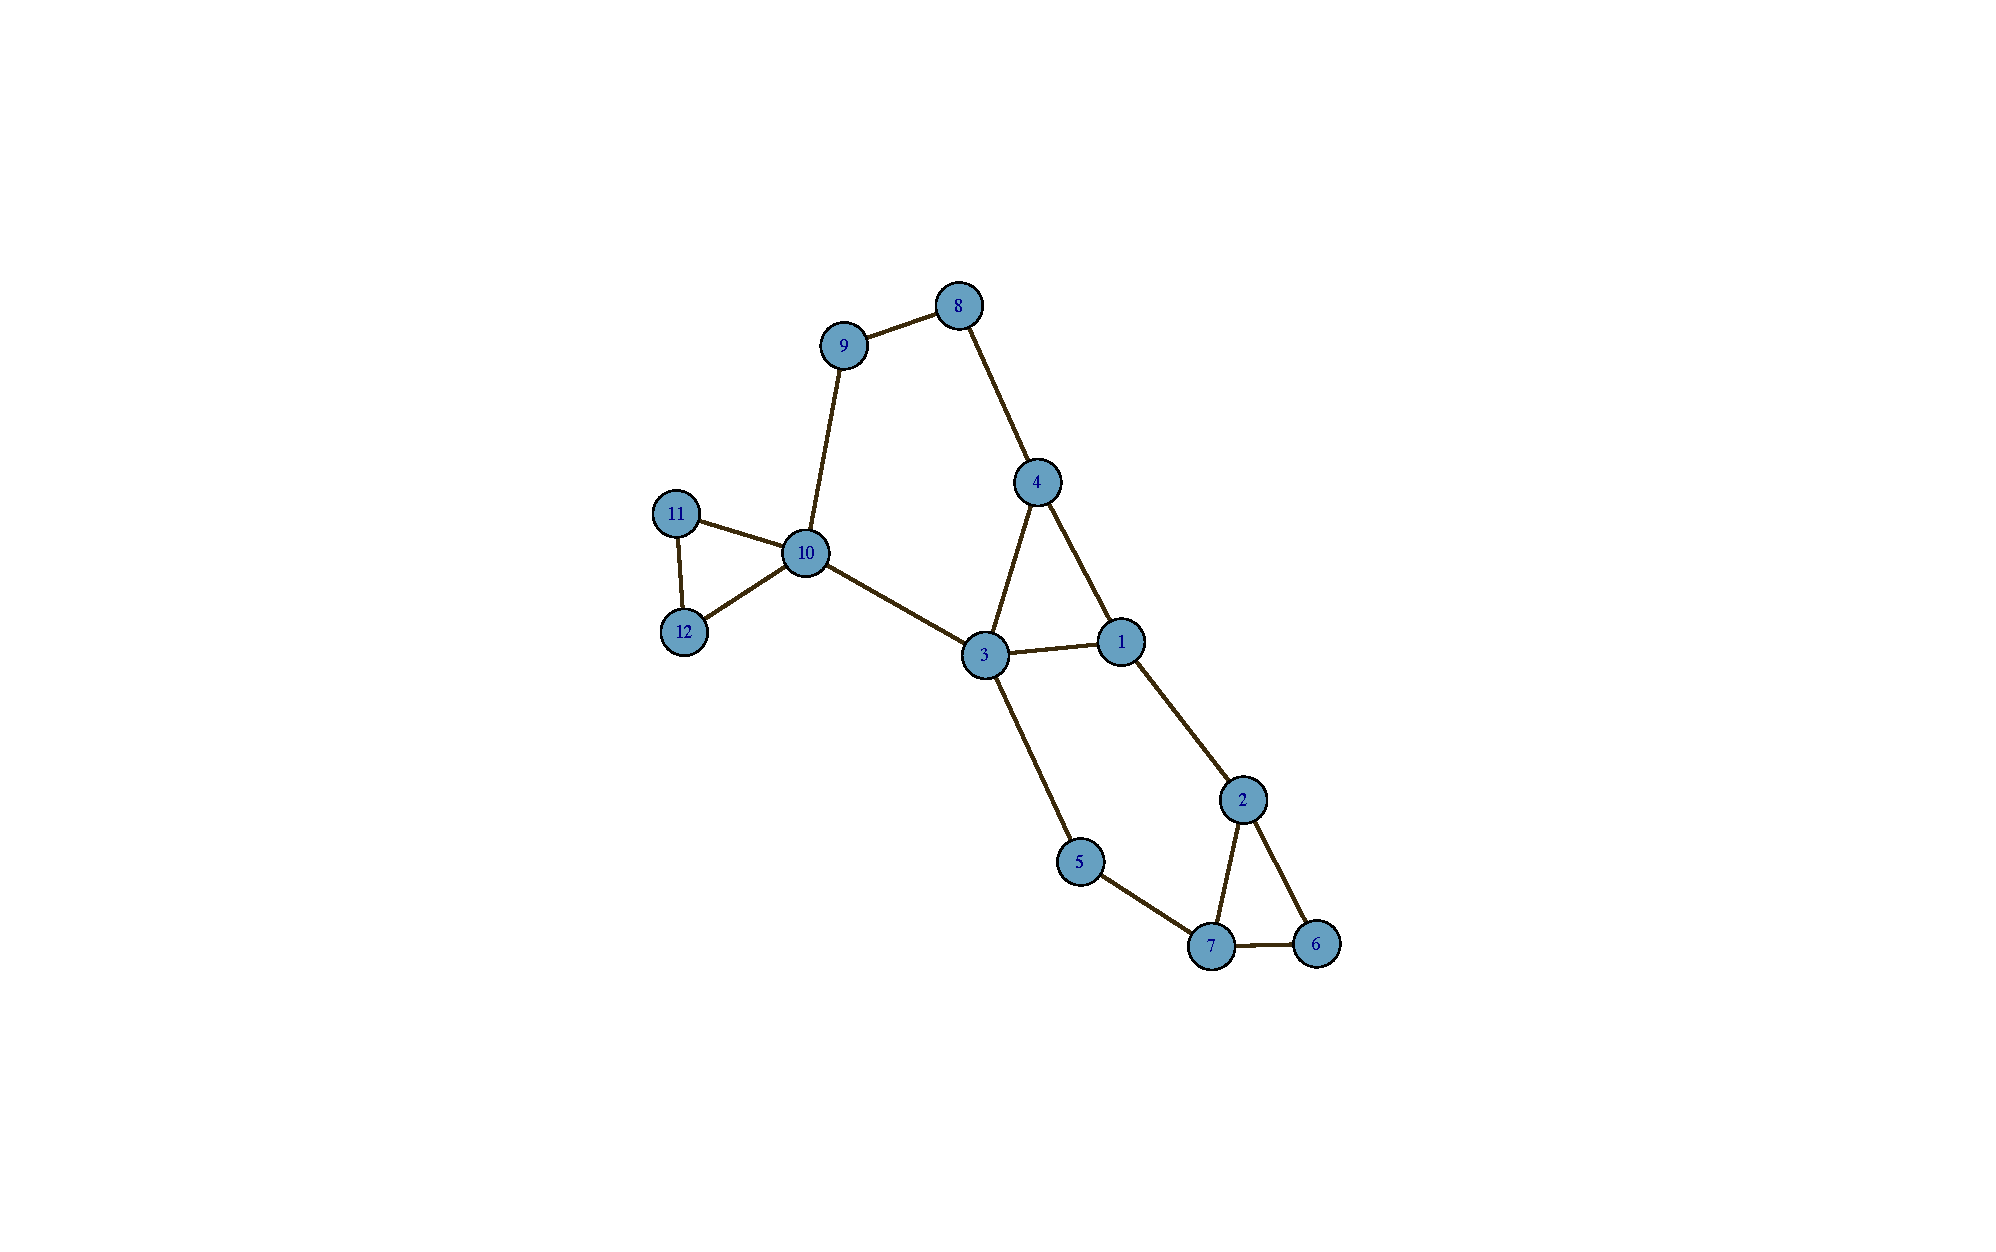
\includegraphics[scale=0.25]{P.pdf}
                \caption{The network used in an example from \cite{Teix2014}}
                \label{fig:TeixierasNetwork}
        \end{subfigure}
        ~ %add desired spacing between images, e. g. ~, \quad, \qquad, \hfill etc.
          %(or a blank line to force the subfigure onto a new line)
        \centering
        \begin{subfigure}[b]{0.25\textwidth}
                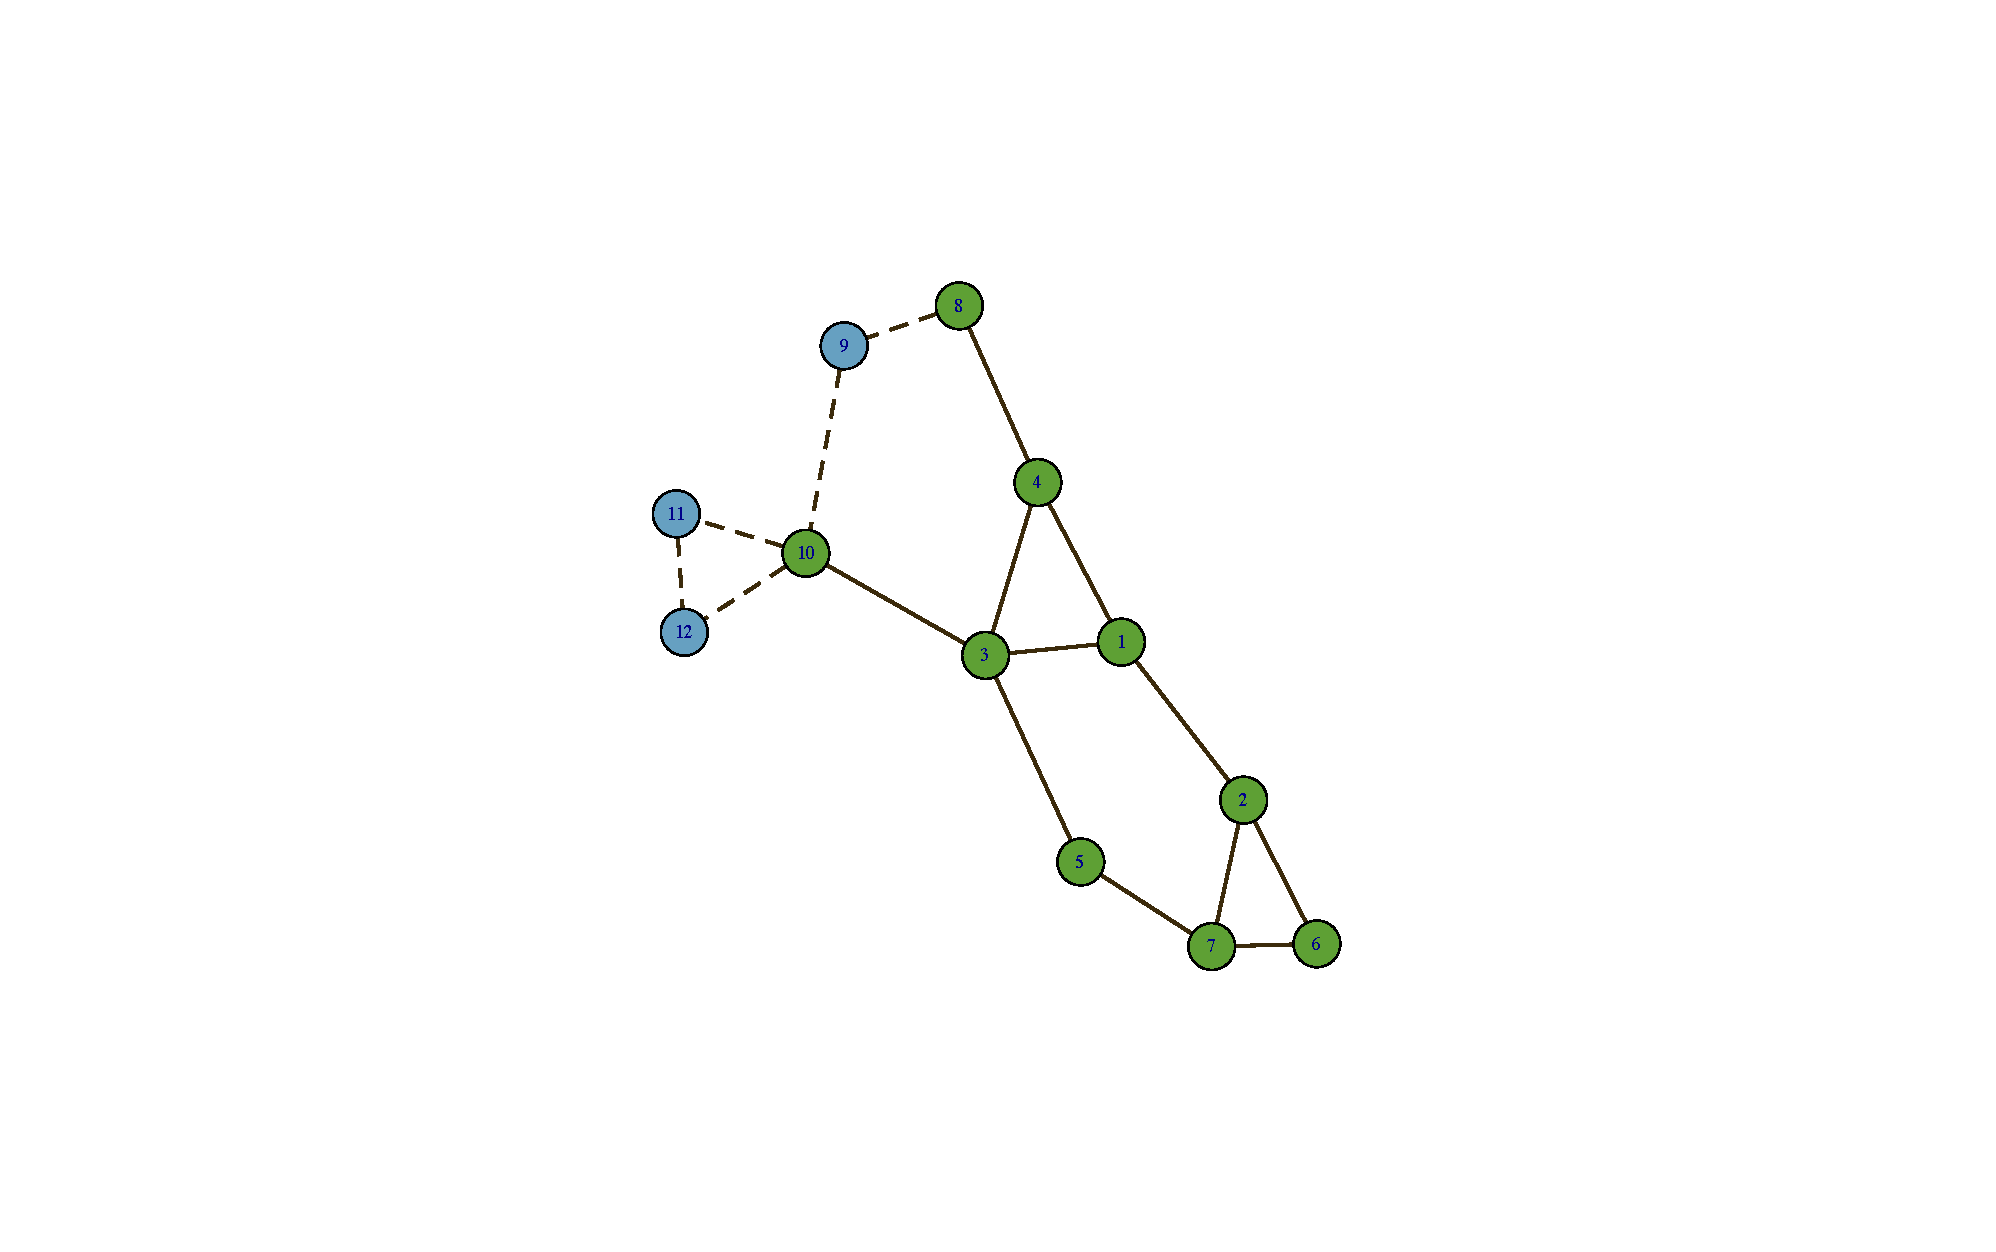
\includegraphics[scale=0.25]{Pmonitoring.pdf}
                \caption{The monitoring agents are shaded green.}
                \label{fig:monitoringagents}
        \end{subfigure}
        ~ %add desired spacing between images, e. g. ~, \quad, \qquad, \hfill etc.
          %(or a blank line to force the subfigure onto a new line)
        \begin{subfigure}[b]{0.25\textwidth}
                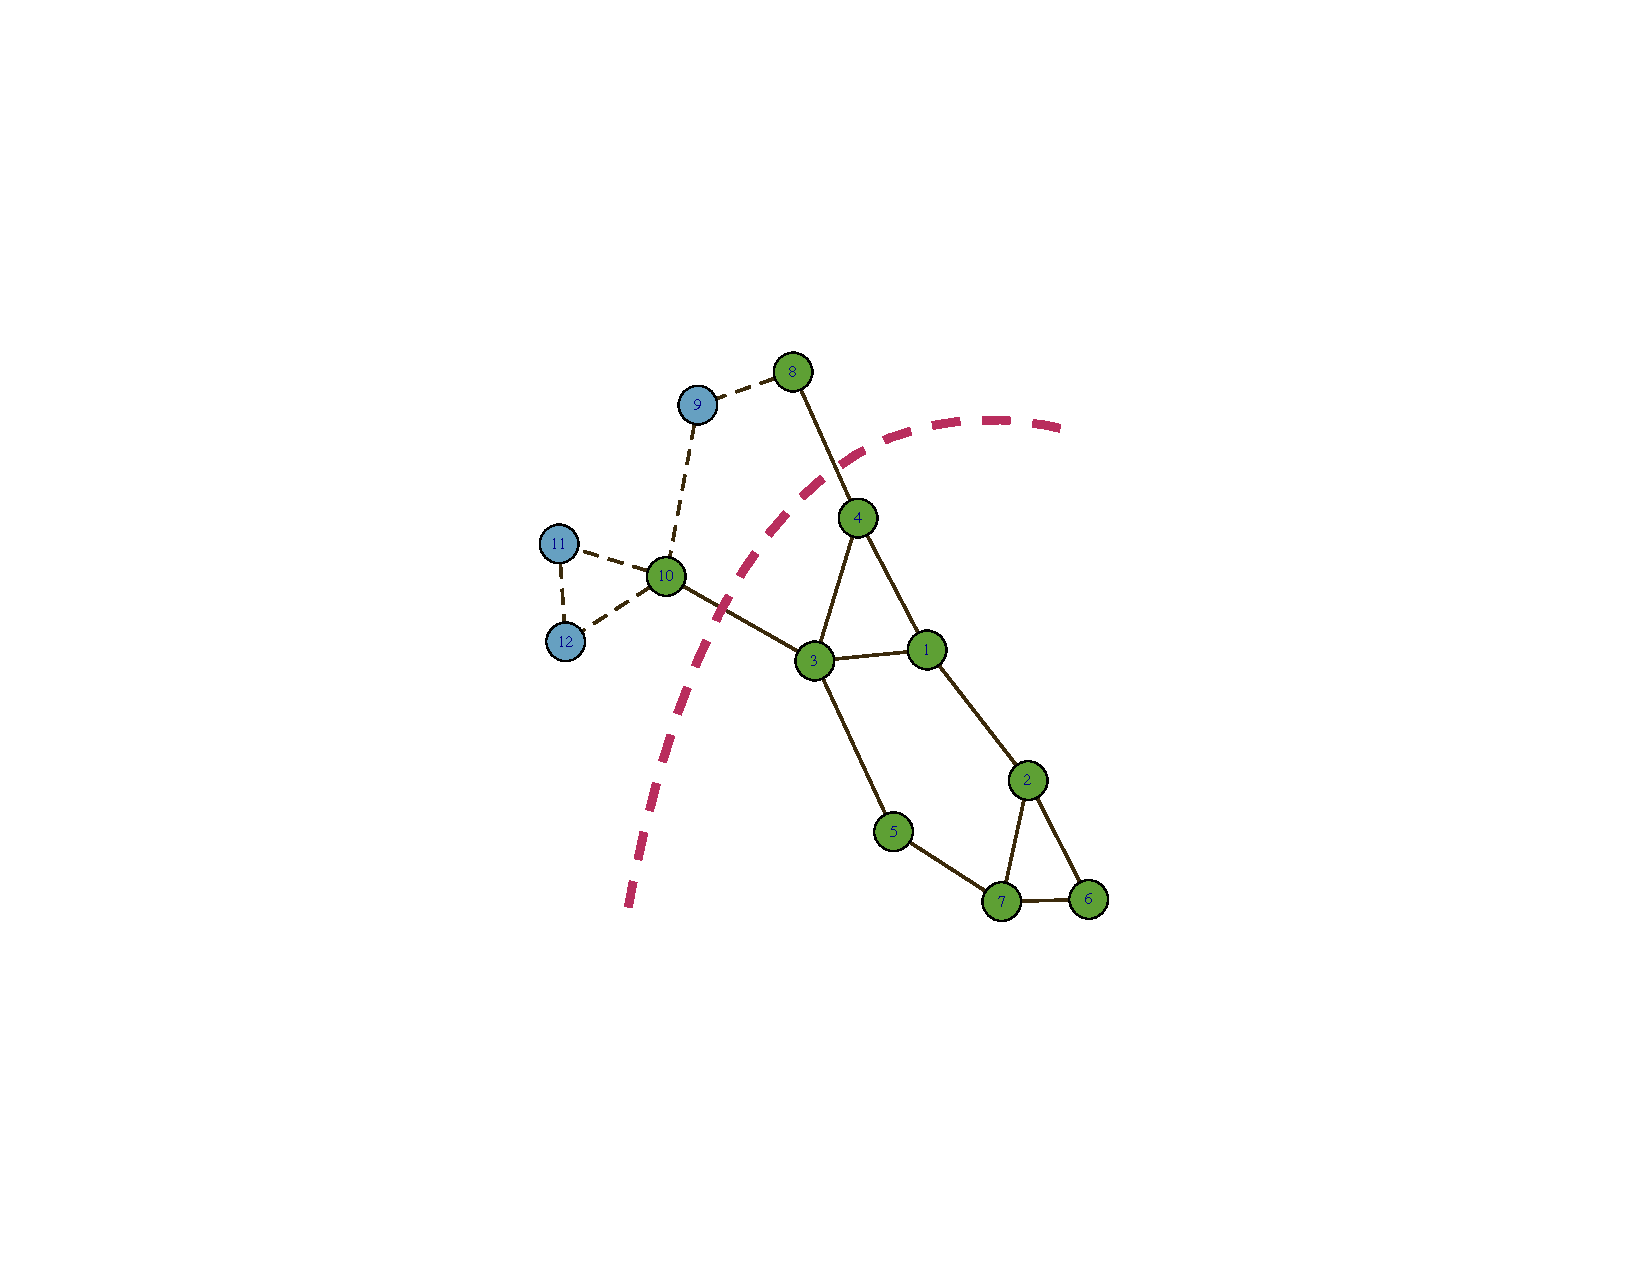
\includegraphics[scale=0.25]{PmonCut.pdf}
                \caption{The attack from the external adversary is shown with red dashed lines.}
                \label{fig:adversaryCut}
        \end{subfigure}
        \caption{}\label{fig:TeixierasNetworkCut}
\end{figure}
\end{center}
\begin{problem}[Spectral Expansion Recovery] \label{pr:p1}
Let $G=(V,E_G)$ be an undirected simple graph and let $H=(V,E_H)$ be a subgraph embedded in $G$. Given $\delta \in \mathbb{R}$, find $S \subset V$ of size $|S| \geq \delta n$ such that

\begin{align} \label{eq:specExpOptim}
\lambda(\delta) = \max_{S:|S|\geq \delta n} \lambda_2(L_H).
\end{align} \qed
\end{problem}
In other words, in Problem \ref{pr:p1} given a parameter $\delta$, we are interested in a subset of the vertices $S\subset V$ of size $|S|\geq \delta n$ with the largest induced spectral expansion.
% \begin{align}\label{eq:benchmarkinducedexp} 
% \lambda(\delta) = \max_{S: |S|\geq \delta n} \lambda_2(H)
% \end{align}
Algorithm \ref{alg:alg1} approximates the set $S \subset \cV$ for which (\ref{eq:specExpOptim}) is satisfied. It returns a set with the largest induced combinatorial expansion for a give $\delta$. 

\medskip
\textcolor{red}{Some notes to consider:}
\begin{itemize}
\item\textcolor{red}{The difficult direction of the Cheeger inequality can be shown by mimicking the approach taken by a) theorem 6.5.1 in Spielmans 2012 lecture 6 notes or Trevisian lecture 4 notes from CS359G blog notes.}
\item\textcolor{red}{However, it may be easier to formulate the theorem in terms of the intruders and the attackers so that it is not a purely mathematical result!}
\item\textcolor{red}{Consider writing the theorem so that $S$ is the set of monitoring agents having the property that their spectral expansion or their combinatorial expansion is beyond some $\epsilon$ etc.}
\item\textcolor{red}{Consider a scenario where the attacker chooses $\delta$ or $\epsilon$ and you choose the other etc.}
\end{itemize}
\begin{theorem}[Existence of Hidden Expander]
Let $G$ be a graph with maximum degree $d_{max}$. For every $0 < \delta,\epsilon < 1$, there exists a set $S \subseteq V$ such that
\begin{align}	
|S| \geq \delta n \quad \text{and} \quad \lambda_2 (H) \geq \epsilon d_{max}
\end{align}
or,
\begin{align}
\frac{\delta}{4}n \leq |S| \leq \delta n \quad \text{and} \quad h(S) \leq (d_{max})\sqrt[]{2 \epsilon}.
\end{align}
\end{theorem}
\begin{proof}
The proof of the theorem simply follows from Cheegers inequality and the fact that for any two disjoint sets, $S$ and $T$, $h(S \cup T) \leq \max{(h(S),h(T))}$. The Laplacian of $G$ is always a PSD matrix by definition. We can write the size of a cut $|E(S,\overline{S})|$ as a quadratic form. For $x=\bone_S$ we get,  
$$
|E(S,\overline{S})|=\bone_S^\intercal L_G \bone_S. 
$$ 
As alluded to earlier, the Cheeger's inequality relates the second eigenvalue of the Laplacian matrix to $h(G)$. The left side of \eqref{eq:cheeger} is known as the \emph{easy} direction, and the the right side is the \emph{hard} direction. The proof of the hard direction follows by a simple rounding algorithm known as the \emph{spectral partitioning algorithm} which rounds the second eigenvector of the Laplacian matrix to a set $S$ of (size $|S|\leq |V|/2)$ and) expansion $O(\sqrt{\lambda_2\cdot \Delta})$. 
For the sake of completeness, here we describe the algorithm:
Let $\bof$ be the second eigenvector of $L_G$. Sort vertices based on $f_v$, and call them $v_1,v_2,\dots,v_n$. Return the best threshold cut, i.e., 
$$ \min_{1\leq i\leq n} \max(h(\{v_1,\dots,v_i\}), h(\{v_{i+1},\dots,v_n\})).$$
%Let $i \in \{1,\ldots,n-1\}$ such that $\max\left( \h(\{v_1,\ldots,v_i\}),\h(\{v_{i+1},\ldots,v_n\})\right )$ is minimal and return $(\{v_1,\ldots,v_i\},\{v_{i+1},\ldots,v_n\})$.
One can use repeated applications of the preceding algorithm to approximate the minimum bisection of a given graph $G$. See \autoref{alg:minbisection} for the details of the algorithm. 
\end{proof}
% \begin{algorithm}
% \begin{algorithmic}
% \State Find a vector $x$ such that $\cR(x) \leq O(\lambda_2)$. One can use power iteration algorithm to find $x$ in linear time but we do not discuss the details.
% \State Sort the vertices of $V$ according to $x$, $x(v_1)\leq x(v_2) \leq \dots\leq x(v_n)$.
% \State {\bf Return} the threshold cut  $(\{v_1,\dots,v_i\},\{v_{i+1},\dots,v_n\})$ with the smallest conductance.
% \end{algorithmic}
% \caption{Spectral Partitioning Algorithm}
% \label{alg:spectralpartitioning}
% \end{algorithm}
\begin{algorithm} 
    \SetKwInOut{Input}{Input}
    \SetKwInOut{Output}{Output}

    %\underline{function Euclid} $(a,b)$\;
    \Input{A graph $G=(V,E)$, with any vector $l \in \R^{\cV}$}
    \Output{A cut $\partial (S)$ in $G$ and $k \in \N$}
    Sort the vertices of $G$ according to the values of $l_{v}$. \\ 
    Find a $k \in \N$ that minimizes $h(\{v_1,\ldots,v_k\},\{v_{k+1},\dots,v_n\})$ and output the index $k$ of $v_k$. 
    \caption{Spectral Partitioning Algorithm}\label{alg:alg0}
\end{algorithm}

\begin{remark}
If $l \in \R^{\cV}$ is an eigenvector of $\lambda_2 (G)$, then Algorithm \ref{alg:alg0} is an efficient and accurate approximation of $h(G)$ in that it can be implemented with time complexity $\mathcal{O}(\mid \cE \mid + \mid \cV \mid log \mid \cV \mid )$. 
\end{remark}
Our main result finds the hidden expander, $H$, embedded in $G$.
\begin{algorithm} 
    \SetKwInOut{Input}{Input}
    \SetKwInOut{Output}{Output}

    %\underline{function Euclid} $(a,b)$\;
    \Input{A graph $G=(V,E)$ with maximum degree $\Delta$ and $0 < \epsilon < 1$.}
    \Output{A set $S$ such that,either $|S| \geq \frac{3}{4}n$ and $\lambda_2 (G[S]) \geq \epsilon \Delta$, or $\frac{n}{4} \leq |S| \leq \frac{3}{4}n$ and $h(S) \leq \sqrt{2\epsilon}\Delta$ }
    Let $S=V$. \\ %\eIf{$b=0$}
    \While{$|S| \geq \frac{3}{4}n$}
    	{If $\lambda_2 (G[S]) \geq \epsilon \Delta$ then \Return{S}.\\ Otherwise, run the spectral partitioning on $G[S]$ and let $(T,S \setminus T)$ be the output. \\ Say $|T| < |S \setminus T|$. Let $S = S \setminus T$.}
 	\Return{$V \setminus S$}
    \caption{Spectral Bisection Algorithm}\label{alg:alg1}
\end{algorithm}

\subsection{Explicit Constructions}
\textcolor{red}{Paley and LBC constructions for $H$, then proof of result in abstract.} 

% %-----------Illustrative Example------------
\section{Illustrative Example}
Example

% %-----------Conclusion------------
\section{Conclusion}
conclude
% %-----------BASICS-------------
% \section{Conclusion}

% \begin{figure}
%     \centering
%         \begin{minipage}{0.45\textwidth}
%             \centering
%             \includegraphics[scale=0.5]{lineGraph2Vertices.png} % first figure itself
%             \caption{Graph X}
%             \label{fig:graphX}
%         \end{minipage}\hfill
%         \begin{minipage}{0.45\textwidth}
%             \centering
%             \includegraphics[scale=0.5]{lineGraph3Vertices.png} % second figure itself
%             \caption{Graph Y}
%             \label{fig:graphY}
%         \end{minipage}
% \end{figure}

\bibliography{thesisBib}
\bibliographystyle{amsplain}
\end{document}
